\documentclass[a4paper]{article}

%% Language and font encodings
\usepackage[english]{babel}
\usepackage[utf8x]{inputenc}
\usepackage[T1]{fontenc}

%% Sets page size and margins
\usepackage[a4paper,top=3cm,bottom=2cm,left=3cm,right=3cm,marginparwidth=1.75cm]{geometry}

%% Useful packages
\usepackage{amsmath}
\usepackage{graphicx}
\usepackage[colorinlistoftodos]{todonotes}
\usepackage[colorlinks=true, allcolors=blue]{hyperref}

\title{Navigation Function}
\author{EdXian}

\begin{document}
\maketitle



\section{Introduction}

An introduction to robot motion planning implemented by potential field approach with navigation function.

\section{Navigation Function}

{\huge $\phi =\frac { { \gamma  } }{ { \left( { \gamma  }^{ k }+\beta  \right)  }^{ 1/k } } $}

\begin{figure}
\centering
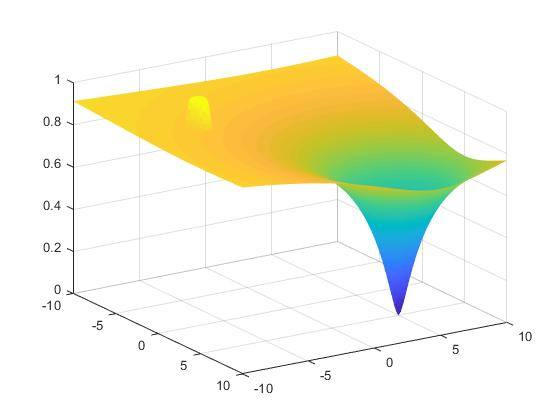
\includegraphics[width=1\textwidth]{potential2.jpg}
\caption{\label{fig:Potential filed}This figure shows the potential field caused by navigation function.}
\end{figure}

\subsection{Goal Function}

 {\Large $\gamma \quad =\quad { \left\| p-{ C }_{ v } \right\|  }^{ 2 } $}


\subsection{Obstacle Avoidance Function}

{\Large $\beta =\frac { 1 }{ 1+{ e }^{ -\left( \left\| { p }_{ io } \right\| -\frac { R }{ { k }_{ 1 } }  \right) \left( \frac { { k }_{ 2 } }{ R }  \right)  } } $}

\subsection{Dynamics}

{\Large $u=-K{ \nabla  }_{ p }\phi $}


\section{Simulation}


\subsection{Qt}

\begin{figure}
\centering
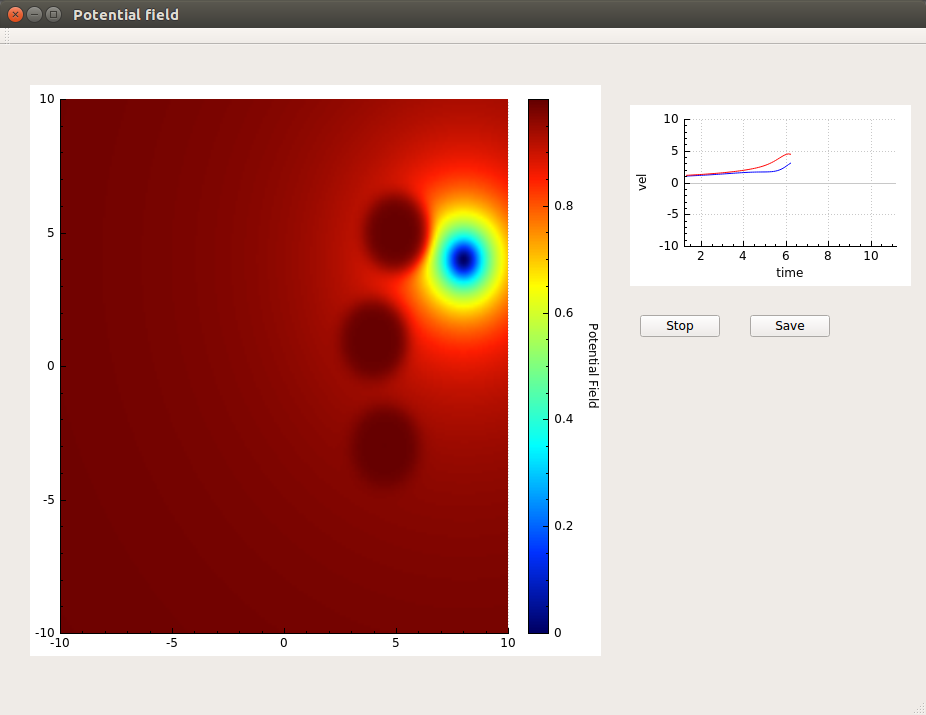
\includegraphics[width=1\textwidth]{colormap.png}
\caption{\label{fig:Colormap}This figure shows the the potential field by colormap.}
\end{figure}

\subsection{Matlab}


\section{Repository}

You can find the resource in my \href{https://github.com/EdXian/Potential-Field-Navigation-Function}{Repository}.

\bibliographystyle{alpha}
\bibliography{sample}

\end{document}\grid
\grid
